% template-v1.tex: LaTeX2e template for Usenix papers.
% Version: usetex-v1, 31-Oct-2002
% Revision history at end.

\documentclass[XXX,endnotes]{usetex-v1}
% Choose the appropriate option:
%
% 1. workingdraft:
%
%       For initial submission and shepherding.  Features prominent
%       date, notice of draft status, page numbers, and annotation
%       facilities.  The three supported annotation macros are:
%               \edannote{text}         -- anonymous annotation note
%               \begin{ednote}{who}     -- annotation note attributed
%                 text                          to ``who''
%               \end{ednote}
%               \HERE                   -- a marker that can be left
%                                               in the text and easily
%                                               searched for later
% 2. proof:
%
%         A galley proof identical to the final copy except for page
%         numbering and proof date on the bottom.  Annotations are
%         removed.
%
% 3. webversion:
%
%       A web-publishable version, uses \docstatus{} to indicate
%       publication information (where and when paper was published),
%       and page numbers.
%
% 4. finalversion:
%
%       The final camera-ready-copy (CRC) version of the paper.
%       Published in conference proceedings.  This doesn't include
%       page numbers, annotations, or draft status (Usenix adds
%       headers, footers, and page numbers onto the CRC).
%
% If several are used, the last one in this list wins
%

%
% In addition, the option "endnotes" permits the use of the
% otherwise-disabled, Usenix-deprecated footnote{} command in
% documents.  In this case, be sure to include a
% \makeendnotes command at the end of your document or
% the endnotes will not actually appear.
%

% These packages are optional, but useful
\usepackage{epsfig}     % postscript figures
\usepackage{url}        % \url{} command with good linebreaks

\begin{document}

\title{Wonderful: A Terrific Application and Fascinating Paper}

% document status: submitted to foo, published in bar, etc.
\docstatus{Submitted to Cool Stuff Conference 2002}

% authors.  separate groupings with \and.
\author{
\authname{Your N.\ Here}
\authaddr{Your Department}
\authaddr{Your Institution}
\authaddr{ Your City, State, ZIP}
\authurl{\url{yourname@host.dom}}
\authurl{\url{http://host.dom/yoururl}}
\and
\authname{Name Two}
\authaddr{Two's Institution}
\authurl{\url{two@host.dom}}
%
} % end author

\maketitle

\begin{abstract}
  Your abstract text goes here.  Just a few facts.  Whet our
  appetites.
\end{abstract}

\section{Introduction}

A paragraph of text goes here.  Lots of text.  Plenty of interesting
text.  Lots of text.  Lots of text.  Lots.  \edannote{We can make
  notes here on the workingdraft, after which they must be removed.
  This one is anonymous.}

More fascinating text. Features galore, plethora of promises.
\begin{ednote}{BCM}
  This ednote is marked as mine.
\end{ednote}

\section{This is Another Section}

Some embedded literal typeset code is shown below.  Note that line or
page breaks can occur in the middle of code typeset this way.  To
avoid such line or page breaks, put the code inside a figure
environment instead.

\begin{small}
\begin{verbatim}
int wrap_fact(ClientData clientData,
              Tcl_Interp *interp,
              int argc, char *argv[]) {
    int result;
    int arg0;
    if (argc != 2) {
        interp->result = "wrong # args";
        return TCL_ERROR;
    }
    arg0 = atoi(argv[1]);
    result = fact(arg0);
    sprintf(interp->result,"%d",result);
    return TCL_OK;
}
\end{verbatim}
\end{small}

Now we're going to cite somebody.  Watch for the cite tag.  Here it
comes~\cite{heidrich,perl5,otcl}.  And a bit later we will cite
another one.  Stay tuned~\cite{ousterhout}.

\section{This Section has Sub-Sections}
\label{sec:secs}

This text is the introduction to Section~\ref{sec:secs}.

\begin{figure}[htbp]
\begin{centering}
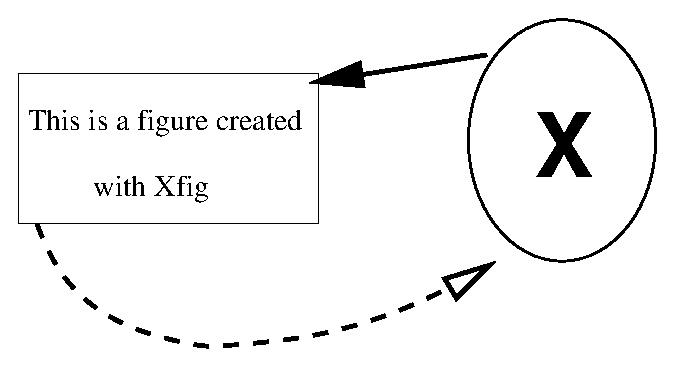
\epsfig{file=sample.eps, width=2.50in}
\small\itshape
\caption{\small\itshape This figure was created with \texttt{xfig}.  If you
want it to span two columns, use \texttt{figure*} in the LaTeX source file.}
\label{fig-sample}
\end{centering}
\end{figure}

\subsection{First Sub-Section}

Here's a typical figure reference.  Figure~\ref{fig:flowchart} is
centered at the top of the column.  It may be scaled.  If so, you may
have to tweak the numbers to get the size you want. It may be
  hard to do this.


\begin{figure}[tb]
  \begin{center}
%    \psfig{file=figure.eps,scale=0.45}         % PostScript figure
     \texttt{<insert figure here>}              % remove this line
    \caption{Wonderful flowchart}
    \label{fig:flowchart}
  \end{center}
\end{figure}

This text came after the figure, so we'll casually refer to
Figure~\ref{fig:flowchart} as we go on our merry way.

% you need to work on the workingdraft document right here soon
\HERE

\subsection{Footnotes}

For the Usenix style, footnotes are not allowed: endnotes
are, although they are
deprecated.\ifhasendnotes\footnote{Thus, this is not a
footnote}\fi\ Try to avoid both footnotes and endnotes in
technical writing.  It is best to use parenthetical or
subordinate clauses instead.  If you want endnotes anyhow,
use the "endnotes" documentstyle option and include a
\verb+\makeendnotes+ command at the end of your document.
You will still be whined at.

\subsection{Tables and Code}

%%%%%%%%%%%%%%%%%%%%%%%%%%%%%%%%%%%%%%%%%%%%%%%%%%%%%%%%%%%%%%%%%%%%%%%%%%%%%%
\begin{table*}[htbp]
\centering
\begin{tabular}{|c||c|c|c|c||c|c|c|c|c|c|l|}\hline
         {\bf Cloak}
        & \multicolumn{4}{c||}{\textbf{User \texttt{ezk}}}
        & \multicolumn{6}{c|}{\textbf{User \texttt{joe}}}
        & \multicolumn{1}{c|}{\textbf{Meaning}}
\\\cline{2-11}
        {\bf Mask}
        &{J1}
        &{J2}
        &{J3}
        &{J4}
        &{E5}
        &{E6}
        &{E7}
        &{E8}
        &{E9}
        &{E10}
        &\multicolumn{1}{c|}{\textbf{for files J1--E10}}
\\\hline
         {+000}
        &
        &
        &
        &
        &
        &
        &
        &
        &
        &
        & Show files to owners only
\\\hline
         {+007}
        &
        &
        &{A}
        &
        &
        &
        &{A}
        &{A}
        &
        &
        & Show files to owners and others
\\\hline
         {+070}
        &
        &{A}
        &{A}
        &
        &{A}
        &
        &{A}
        &{A}
        &
        &
        & Show files to owners and group members
\\\hline
\end{tabular}
\small\itshape
\caption{\small\itshape Here is a complex table that spans two columns.  It
  shows how also to straddle the table cells.}
\label{tab-sample}
\end{table*}
%%%%%%%%%%%%%%%%%%%%%%%%%%%%%%%%%%%%%%%%%%%%%%%%%%%%%%%%%%%%%%%%%%%%%%%%%%%%%%

It can get tricky typesetting Tcl and C code in LaTeX because they
share a lot of mystical feelings about certain magic characters.  You
will have to do a lot of escaping to typeset curly braces and percent
signs, for example, like this: ``The \verb@%module@ directive sets
the name of the initialization function.  This is optional, but is
recommended if building a Tcl 7.5 module.  Everything inside the 
\verb@%{@, \verb@%}@ block is copied directly into the
output. allowing the inclusion of header files and additional C code.''

Sometimes you want to really call attention to a piece of text.  You
can center it in the column like this:
\begin{center}
\verb@_1008e614_Vector_p@
\end{center}
and people will really notice it.

Now this is an ingenious way to get a forced space.  \texttt{Real~$*$}
and \texttt{double~$*$} are equivalent.


\subsection{Lists}

You can make lists using LaTeX's listing environments
(\texttt{itemize}, \texttt{enumerate}, and \texttt{description}).
These environments can be nested (e.g. an itemized list can be an
element of an enumerated list).

An \texttt{itemize} list looks like this:
\begin{itemize}
\item The map structure defines an address space.
\item The page structure manages a page of physical memory.
\end{itemize}

An \texttt{enumerate} list is like an itemized list, except that it is
numbered:
\begin{enumerate}
\item The map structure defines an address space.
\item The page structure manages a page of physical memory.
\end{enumerate}

A \texttt{description} list uses words rather bullets or numbers:
\begin{description}
\item[\textbf{map structure:}] defines an address space.
\item[\textbf{page structure:}] manages a page of physical memory.
\end{description}

\subsection{Last Sub-Section}

Well, it's getting boring isn't it.  This is the last subsection
before we wrap it up.

\section{Acknowledgments}

A polite author always includes acknowledgments.  You
should thank everyone,
especially those who funded the work.

\section{Availability}

It is great news if this section can say that your
app, WonderfulApp is free
software, available via anonymous FTP from
\url{ftp://ftp.dom/pub/myname/Wonderful}.  Also, it's even better
when you can write that information is also available on the Wonderful
homepage at \url{http://www.dom/~myname/SWIG}.

Now we get serious and fill in those references.  Remember you will
have to run latex twice on the document in order to resolve those
cite tags you met earlier.  This is where they get resolved.
We've preserved some real ones in addition to the template-speak.
After the bibliography you are DONE.

% This is where the endnotes (see the ``footnote'' above)
% are filled in.  Use this only if you have endnotes.
\ifhasendnotes\makeendnotes\fi

\begin{thebibliography}{99}

\bibitem{beazley} D.~M.~Beazley and P.~S.~Lomdahl, 
\emph{Message-Passing Multi-Cell Molecular Dynamics on the Connection
Machine 5}, Parall.~Comp.~ 20 (1994) p. 173-195.

\bibitem{CitePetName} A.~N.~Author and A.~N.~Other, 
\emph{Title of Riveting Article}, JournalName VolNum (Year) p. Start-End

\bibitem{embed} Embedded Tk, \url{ftp://ftp.vnet.net/pub/users/drh/ET.html}

\bibitem{expect} Don Libes, \emph{Exploring Expect}, O'Reilly \& Associates, Inc. (1995).

\bibitem{heidrich} Wolfgang Heidrich and Philipp Slusallek, \emph{
Automatic Generation of Tcl Bindings for C and C++ Libraries.},
USENIX 3rd Annual Tcl/Tk Workshop (1995).

\bibitem{ousterhout} John K. Ousterhout, \emph{Tcl and the Tk Toolkit}, Addison-Wesley Publishers (1994).

\bibitem{perl5} Perl5 Programmers reference,
\url{http://www.metronet.com/perlinfo/doc}, (1996).

\bibitem{otcl} D. Wetherall, C. J. Lindblad, ``Extending Tcl for
Dynamic Object-Oriented Programming'', Proceedings of the USENIX 3rd Annual Tcl/Tk Workshop (1995).

\end{thebibliography}

\end{document}

% Revision History:
% designed specifically to meet requirements of
%  TCL97 committee.
% originally a template for producing IEEE-format articles using LaTeX.
%   written by Matthew Ward, CS Department, Worcester Polytechnic Institute.
% adapted by David Beazley for his excellent SWIG paper in Proceedings,
%   Tcl 96
% turned into a smartass generic template by De Clarke, with thanks to
%   both the above pioneers
% use at your own risk.  Complaints to /dev/null.
% make it two column with no page numbering, default is 10 point

% Munged by Fred Douglis <douglis@research.att.com> 10/97 to separate
% the .sty file from the LaTeX source template, so that people can
% more easily include the .sty file into an existing document.  Also
% changed to more closely follow the style guidelines as represented
% by the Word sample file.
% This version uses the latex2e styles, not the very ancient 2.09 stuff.
%

% Revised July--October 2002 by Bart Massey, Chuck Cranor, Erez
% Zadok and the FREENIX Track folks to ``be easier to use and work
% better''. Hah.  Major changes include transformation into a
% latex2e class file, better support for drafts, and some
% layout improvements.
%%%%%%%%%%%%%%%%%%%%%%%%%%%%%%%%%%%%%%%%%%%%%%%%%%%%%%%%%%%%%%%%%%%%%%%%%%%%%%
% for Ispell:
% LocalWords:  workingdraft BCM ednote SubSections xfig SubSection joe
